\section{Introduction}

Given a binary relation $R$ such that is:
\begin{itemize}
    \item Reflexive: $a R a$
    \item Symmetric: $a R b \Rightarrow b R a$
    \item Transitive: $a R b \land b R c \Rightarrow a R c$
\end{itemize}

we say that $R$ provides a partition $\Pi$ of $A$ into disjoint equivalence classes. That is, $\Pi = \{A_1, \ldots, A_k\}$ is defined as follows:

\begin{itemize}
    \item $\forall A_i, A_j \in \Pi, A_i \cap A_j = \emptyset \iff A_i \neq A_j$
    \item $A = \bigcup\limits_{i = 1}^{k} A_i$
    \item $a \equiv b \iff a,b \in A_i$ for some $A_i \in \Pi$.
\end{itemize}


Such idea was used in Computer Science by Galler and Fisher\cite{galler1964improved} as the \textbf{union-find data structure} which is a data structure that stores partition of a set into disjoint sets. In particular \textbf{union find} consist of two main operation:

\begin{itemize}
    \item Find Operation: Given two elements $a,b \in A$ determine if $\exists A_i \in \Pi$ s.t $a,b \in A_i$.
    \item Union Operation: Given two elements $a \in A_i$ and $b \in A_j$, \textit{merge} $A_i$ and $A_j$. That is, the result of this operation to the partition $\Pi$ will be a new partition $\Pi'$ such that $\Pi' = (\Pi \setminus \{A_i, A_j\}) \cup (A_i \cup A_j)$.
\end{itemize}

\section{Implementation}
From now on we are going to assume that our set $A$ is defined as $\{0, \ldots, n-1\}$ (and if it is not the case we can use a dictionary to map elements from $A$ to that range).

\subsection{Representation of the partition}
As every subset defines an equivalence class it is equivalent to represent every $A_i \subseteq A$ with a single element $a \in A_i$ which is called the \textit{representative} of $A_i$ (every other element of $A_i$ will be related to $a$ by the properties of the binary relation previously defined). Hence, in our union-find data structure every element will either the representative of a certain subset of $A$ or it will point to someone who is in the same subset (later on different techniques will be discussed to see which is the best element "to point" and what that means). 

A union-find data structure consists of an array $v[0:n-1]$ and every element $i \in A$ will either point to another element $j \in A$ such that they both belong to the same class (in that case $v[i] = j$) or $i$ will be the representative of a certain class and it will be marked \textit{specially}.

\begin{figure}
    \centering
    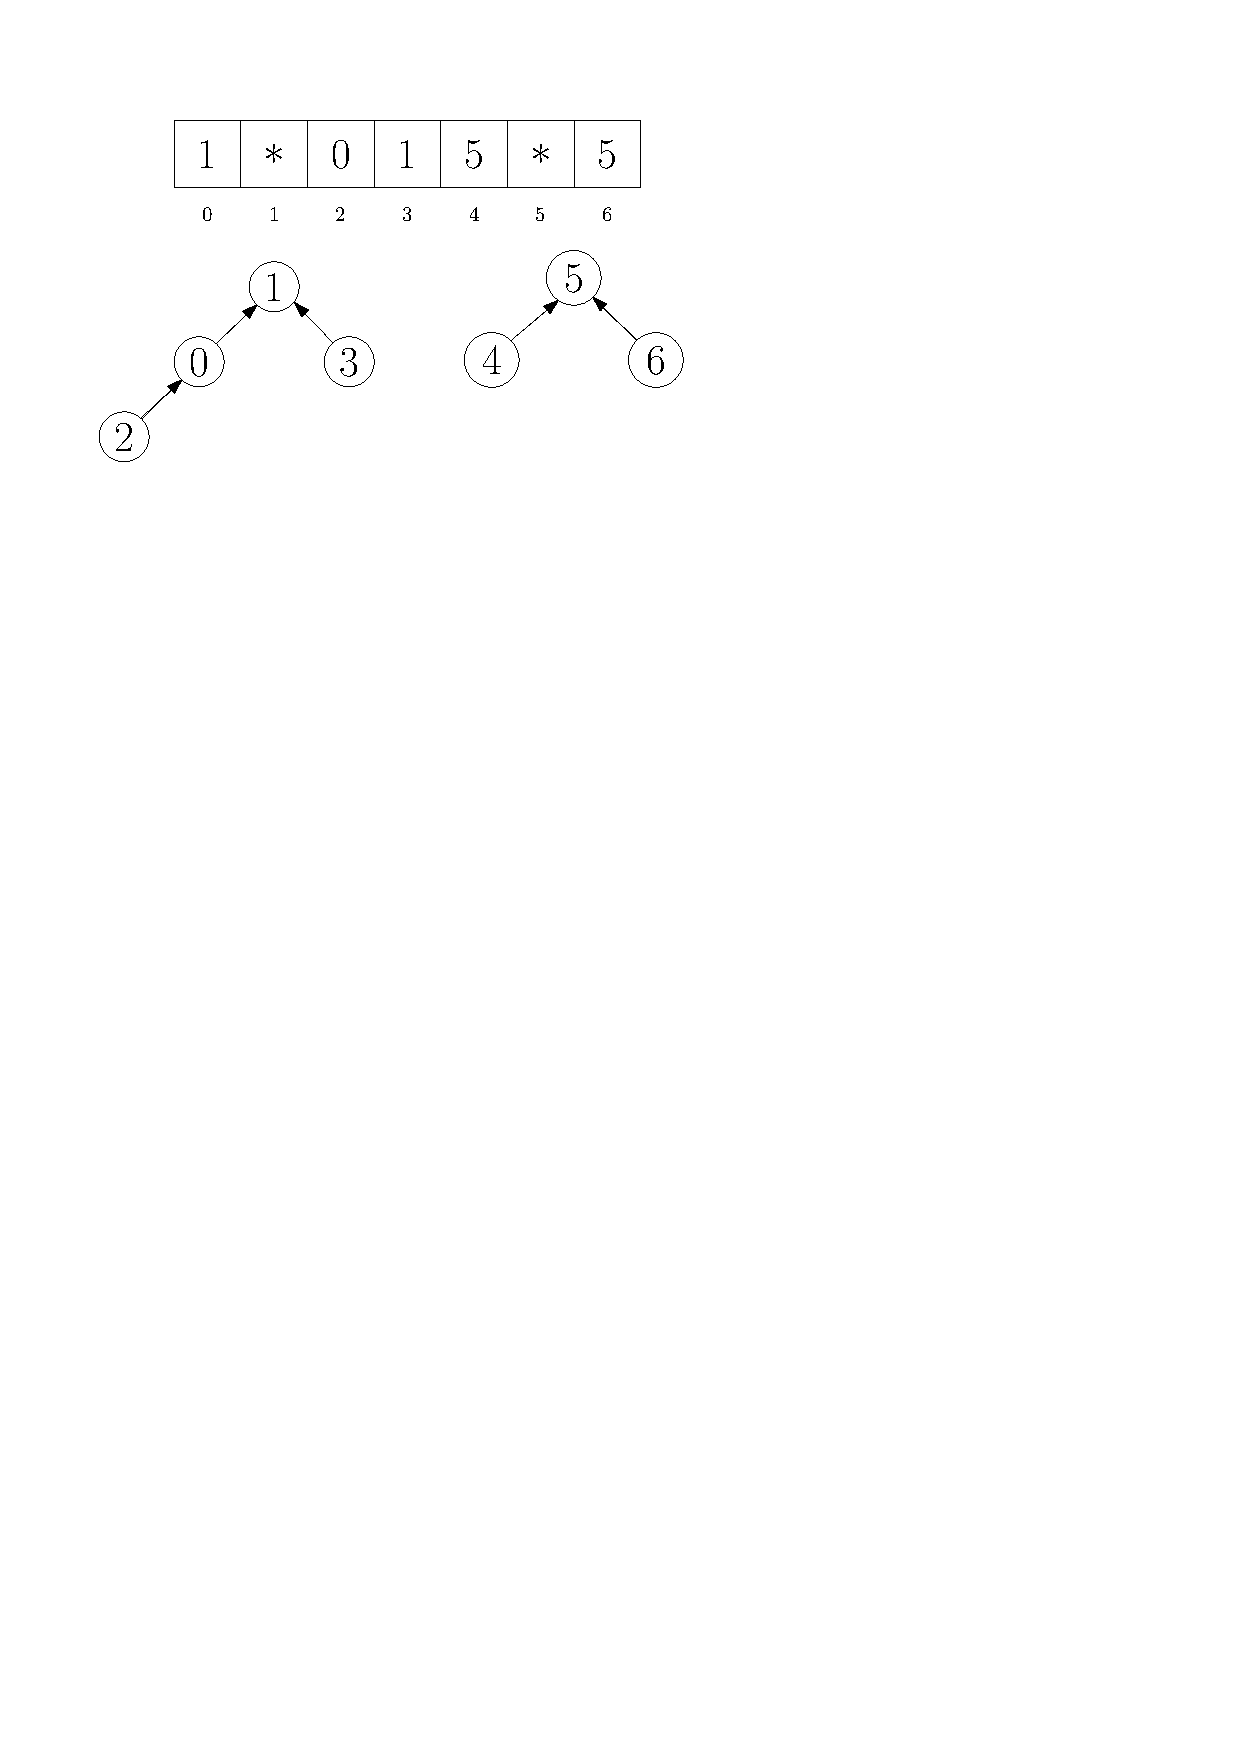
\includegraphics[scale=0.75]{images/ufExample.pdf}
    \caption{An example of a representation of a Union-Find}
\end{figure}
